\documentclass[10pt]{article}
\usepackage[a4paper]{geometry}
\usepackage[linesnumbered,ruled]{algorithm2e}
\usepackage{amsmath}
\usepackage{amssymb}
\usepackage{tocbibind}
\usepackage{graphicx}
\usepackage{hyperref}
\usepackage{mdframed}
\usepackage{subfiles}
\usepackage{titlesec}
\usepackage[dvipsnames]{xcolor}

%%%%%%%%%%%%%%%%%%%%%%%%%%%%%%%%%%%%%%%%%%%%%%%%%%%%%%%%%%%%%%%%%%%%%%%% Setups
\newcommand{\Eq}[1]{Equation~\ref{eq:#1}}
\newcommand{\Fig}[1]{Figure~\ref{fig:#1}}

\newcommand{\Eg}{\textit{e.g.}}
\newcommand{\Ie}{\textit{i.e.}}
\newcommand{\Etc}{\textit{etc.}}

\newenvironment{textbox}[1]
{%
  \mdfsetup{%
    frametitle={\colorbox{white}{\space#1\space}},
    frametitleaboveskip=-\ht\strutbox,
  }
  \begin{mdframed}
}
{
  \end{mdframed}
}

\setlength\parindent{0pt}
\setlength\parskip{1.2ex}

\graphicspath{{./fig/}}

\hypersetup{%
  hidelinks,
  colorlinks,
  citecolor={YellowOrange!85!black},
  linkcolor={Aquamarine!85!black},
  bookmarksopen=true,
  bookmarksnumbered=true,
  linktoc=all,
  pdfauthor=Jihang Li,
}

\title{Notes of ``Configurable 3D scene Synthesis and 2D Image Rendering with
Per-Pixel Ground Truth using Stochastic Grammars''}
\author{Jihang Li}
%%%%%%%%%%%%%%%%%%%%%%%%%%%%%%%%%%%%%%%%%%%%%%%%%%%%%%%%%%%%%%%%%%%%%%%%%%%%%%%

\begin{document}
\maketitle
\tableofcontents

%%%%%%%%%%%%%%%%%%%%%%%%%%%%%%%%%%%%%%%%%%%%%%%%%%%%%%%%%%%%%%%%%%%%%% Abstract
\section*{Abstract}%
\label{sec:abstract}
Devising a learning-based pipeline of algorithms capable of automatically
generating and rendering a potentially infinite variety of indoor scenes by
using a stochastic grammar, represented as an attributed Spatial And-Or
Graph, in conjunction with SOTA PBR\@.

Synthesizing detailed, per-pixel ground truth data:
%
\begin{itemize}
  \item surface depth
  \item surface normal
  \item object identity
  \item material information (detailed to object parts)
  \item environments (\Eg, illuminations and camera viewpoints)
\end{itemize}


%%%%%%%%%%%%%%%%%%%%%%%%%%%%%%%%%%%%%%%%%%%%%%%%%%%%%%%%%%%%%%%%%%%%% Chapter 1
\section{Introduction}%
\label{sec:introduction}
Current RGB-D dataset limitations:
%
\begin{enumerate}
  \item Insufficient labeled RGB-D pairs (\Eg, NYU-Depth V2).
  \item Manual labeling of per-pixel ground truth information is tedious and
    error prone.
\end{enumerate}

This work is unique in devising a complete \textbf{learning-based} pipeline for
synthesizing large scale \textit{learning-based configurable} scene layouts via
stochastic sampling with PBR of these scenes with associated per-pixel ground
truth. This pipeline has the characteristics:
%
\begin{itemize}
  \item By utilizing an attributed S-AOG, the sampling algorithm combines
    \textbf{hierarchical compositions} and \textbf{contextual constraints} to
    enable the generation of 3D scenes with high variability.
  \item As shown in \Fig{1}, SOTA PBR is employed.
\end{itemize}
%
\begin{figure}[!htpb]
  \centering
  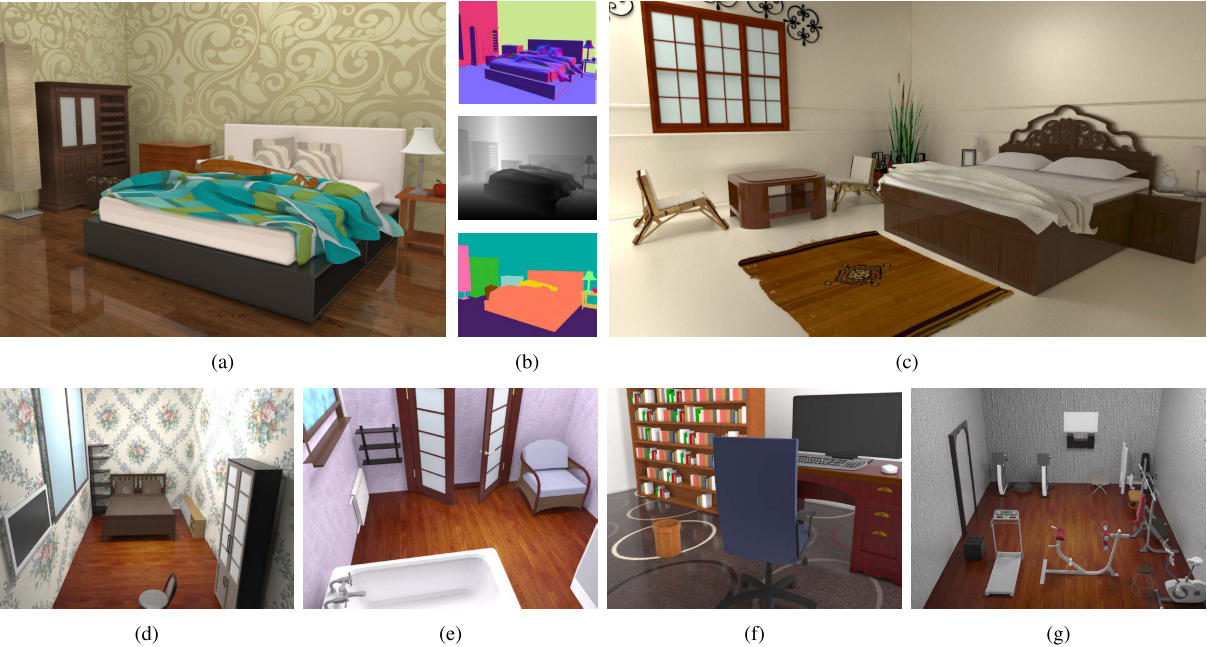
\includegraphics[width=0.9\linewidth]{fig_1.png}
  \caption{(a) An example automatically-generated 3D bedroom scene, rendered as
    a photorealistic RGB image, along with its (b) per-pixel ground truth (from
    top) surface normal, depth, and object identity images. (c) Another
    synthesized bedroom scene. Synthesized scenes include fine details ---
    objects (\Eg, duvet and pillows on beds) and their textures are changeable,
    by sampling the physical parameters of materials (reflectance, roughness,
    glossiness, \Etc.), and illumination parameters are sampled from continuous
    spaces of possible positions, intensities, and colors. (d) – (g) Rendered
    images of four other example synthetic indoor scenes --- (d) bedroom, (e)
    bathroom, (f) study, (g) gym.}%
  \label{fig:1}
\end{figure}

Since the synthesizing is in a forward manner --- by rendering 2D images from
3D scenes containing detailed geometric object models --- ground truth
information is naturally available.

Contributions:
%
\begin{enumerate}
  \item The first work that, for the purposes of indoor scene understanding,
    introduces a \textit{learning-based configurable} pipeline for generating
    massive photorealistic images and indoor scenes with per-pixel ground truth.
  \item Propose S-AOG for scene generation, which supports \textbf{arbitrary
    addition and deletion} of objects and \textbf{modification} of their
    categories.
  \item The first work to provide comprehensive diagnostics w.r.t.\ algorithm
    stability and sensitivity to certain scene attributes.
  \item Demonstrate the effectiveness of the synthesized scene dataset by
    advancing the SOTA in the prediction of surface normal and depth from RGB
    images.
\end{enumerate}


%%%%%%%%%%%%%%%%%%%%%%%%%%%%%%%%%%%%%%%%%%%%%%%%%%%%%%%%%%%%%%%%%%%%% Chapter 2
\section{Representation and Formulation}%
\label{sec:representation_and_formulation}
%================================================================== Section 2.1
\subsection{Representation: Attributed Spatial And-Or Graph}%
\label{sec:representation}
A scene model should be capable of (i) representing the
compositional/hierarchical structure of indoor scenes, and (ii) capturing the
rich contextual relationships between different components of the scene:
%
\begin{itemize}
  \item Compositional hierarchy models the decomposition into sub-components
    and the switch among multiple alternative sub-configurations.
  \item Contextual relations:
    %
    \begin{itemize}
      \item between furniture and walls
      \item among furniture
      \item between supporting and supported objects
      \item between objects of a functional pair
    \end{itemize}
\end{itemize}

\textbf{Representation:}

An attributed S-AOG, which is a \textbf{Stochastic Context-Sensitive Grammar
(SCSG)}, combines:
%
\begin{itemize}
  \item a \textbf{stochastic context-free grammar (SCFG)}
  \item contextual relations defined on a \textbf{Markov random field (MRF)}
\end{itemize}

\textbf{Definitions:}

An S-AOG is defined as a 5-tuple: $\mathcal{G} = \langle S, V, R, P, E \rangle$,
where:
%
\begin{itemize}
  \item $S$: the root node of the scene grammar
  \item $V$: the vertex set
    \begin{itemize}
      \item $V = V_{NT} \cup V_T$
      \item $V_{NT} = V^{And} \cup V^{Or} \cup V^{Set}$\footnote{$V^{Set}$: A
          set of Or-nodes serving as child branches are grouped by an And-node,
          and each child branch may include different numbers of objects.}
      \item $V_T = V^r_T \cup V^a_T$
        \begin{enumerate}
          \item Regular terminal node: $v \in V^r_T$, represents a spatial
            entity in a scene with \textbf{internal attributes} of object sizes
            $(w, l, h)$, and \textbf{external attributes} $A_{ext}$ of
            object position $(x, y, z)$ and orientation ($x - y$ plane)
            $\theta$ and sampled human positions.
          \item Address terminal node: $v \in V^a_T$, encodes interactions that
            only occur in a certain context but a absent in all others; point
            to $v \in V^r_T$ and take values in $V^r_T \cup \{\text{nil}\}$.
        \end{enumerate}
    \end{itemize}
  \item $R$: the production rules
    %
    \begin{itemize}
      \item And rules for $v \in V^{And}$:
        %
        \begin{align}
          \label{eq:1}
          v \rightarrow u_1 \cdot u_2 \cdot \ldots \cdot u_{n(v)}.
        \end{align}
        %
      \item Or rules for $v \in V^{Or}$:
        %
        \begin{align}
          \label{eq:2}
          v \rightarrow u_1 \vert u_2 \vert \ldots \vert u_{n(v)},
        \end{align}
        %
        with $\rho_1 \vert \rho_2 \vert \ldots \vert \rho_{n(v)}$.
      \item Set rules for $v \in V^{Set}$:
        %
        \begin{align}
          \label{eq:3}
          v \rightarrow (\text{nil} \vert u^1_1 \vert u^2_1 \vert \ldots) \dots (\text{nil} \vert u^1_{n(v)} \vert u^2_{n(v)} \vert \ldots),
        \end{align}
        %
        with $(\rho_{1,0} \vert \rho_{1,1} \vert \rho_{1,2} \vert \ldots) \ldots (\rho_{n(v),0} \vert \rho_{n(v),1} \vert \rho_{n(v),2} \vert \ldots)$,
        where $u^k_i$ denotes that object $u_i$ appear $k$ times, and the
        probability is $\rho_{i,k}$.
    \end{itemize}
    %
  \item $P$: the probability model
  \item $E$: the contextual relations, $E = E_f \cup E_o \cup E_g \cup E_w$
    \begin{itemize}
      \item $E_f$: relations among furniture
      \item $E_o$: relations between supported objects and their supporting
        objects
      \item $E_g$: relations in a functional pair
      \item $E_w$: relations between furniture and walls\footnote{This is
        different from $E_r$ in ``Human-centric Indoor Scene Synthesis Using
        Stochastic Grammar'' (hereinafter referred to as ``Human-centric
        Synthesis'').}
    \end{itemize}
    $E$ inherited from their parents; hence the relations at a higher level
    will eventually collapse into cliques $C = C_w \cup C_f \cup C_o \cup C_g$
    among the $v \in V_T$. $E$ also form an MRF on $v \in V_T$.
\end{itemize}

A $pt$ instantiates the S-AOG by selecting a child node for $V^{Or}$ as well as
determining the state of each child node for the $V^{Set}$. And
$pg = (pt, E_{pt})$.

%================================================================== Section 2.2
\subsection{Probabilistic Formulation}%
\label{sec:formulation}
The \textbf{prior probability} of $pg$ generated by an S-AOG parameterized by
$\Theta$ is formulated as a Gibbs distribution\footnote{\label{note3}The style
of ``E'' and ``$\Theta$'' are different from those in the original paper, but
consistent with those in ``Human-centric Synthesis'' for the convenience of
comparison.}:
%
\begin{align}
  p(pg \vert \Theta) &= \frac{1}{Z} \exp (-\mathcal{E}(pg \vert \Theta)) \label{eq:4} \\
                     &= \frac{1}{Z} \exp (-\mathcal{E}(pt \vert \Theta) - \mathcal{E}(E_{pt} \vert \Theta)), \label{eq:5}
\end{align}
%
where:
%
\begin{itemize}
  \item $\mathcal{E}(pg \vert \Theta)$: the energy function of a $pg$
  \item $\mathcal{E}(pt \vert \Theta)$: the energy function of a $pt$
  \item $\mathcal{E}(E_{pt} \vert \Theta)$: the energy term of the contextual
    relations
\end{itemize}
%
$\mathcal{E}(pt \vert \Theta)$ can be decomposed into:
%
\begin{align}
  \label{eq:6}
  \mathcal{E}(pt \vert \Theta) = \underbrace{\sum_{v \in V^{Or}} \mathcal{E}^{Or}_{\Theta}(v) + \sum_{v \in V^{Set}} \mathcal{E}^{Set}_{\Theta}(v)}_{\text{non-terminal nodes}} + \underbrace{\sum_{v \in V^r_T} \mathcal{E}^{A_{in}}_{\Theta}(v)}_{\text{terminal nodes}},
\end{align}
%
where the choice of the child node of an $v \in V^{Or}$ and the child branch of
a $v \in V^{Set}$ follows a \textbf{Bernoulli distribution}. $A_{in}$
of $V_T$ follows a non-parametric probability distribution learned by
\textbf{kernel density estimation}. Note that the $v \in V^{And}$ are
deterministically expanded; hence \Eq{6} lacks an energy term for $V^{And}$.

$\mathcal{E}(E_{pt} \vert \Theta)$ combines the potentials of the 4 types of
cliques which are computed based on $A_{ex}$ of $V^r_T$:
%
\begin{align}
  p(E_{pt} \vert \Theta) &= \frac{1}{Z} \exp (-\mathcal{E}(E_{pt} \vert \Theta)) \label{eq:7} \\
                         &= \prod_{c \in C_w} \phi_w(c) \prod_{c \in C_f} \phi_f(c) \prod_{c \in C_o} \phi_o(c) \prod_{c \in C_g} \phi_g(c). \label{eq:8}
\end{align}
%
where:
%
\begin{itemize}
  \item $\phi_w(c)$:
    %
    \begin{align}
      \label{eq:9}
      \phi_w(c) = \frac{1}{Z} \exp\biggl( -\lambda_w \cdot \left\langle \underbrace{\sum_{w_i \neq w_j} l_{con}(w_i, w_j)}_{\text{constraint between walls}}, \underbrace{\sum_{w_i}[l_{dis}(f, w_i) + l_{ori}(f, w_i)]}_{\text{constraint between walls and furniture}} \right\rangle \biggr),
    \end{align}
    %
    where:
    %
    \begin{itemize}
      \item $c = \{f, \{w_i\}\}$: a clique includes a terminal node
        representing a furniture $f$ and terminal nodes representing $\{w_i\}$.
      \item $\lambda_w$: a weight vector.
      \item $l_{con}(w_i, w_j)$: defines the consistency between the walls;
        \Ie, adjacent walls should be connected, whereas opposite walls should
        have the same size. \textbf{It is usually zero as the walls are
        enforced to be consistent in practice.}
      \item $l_{dis}(x_i, x_j)$: defines the geometric distance compatibility
        between two objects
        %
        \begin{align}
          \label{eq:10}
          l_{dis}(x_i, x_j) = \lvert d(x_i, x_j) - \bar{d}(x_i, x_j) \rvert,
        \end{align}
        %
        where $d(x_i, x_j)$ is the distance between object $x_i$ and $x_j$, and
        $\bar{d}(x_i, x_j)$ is the \textbf{mean distance} learned from all the
        examples.
      \item $l_{ori}(x_i, x_j)$: defines the relative orientation compatibility
        %
        \begin{align}
          \label{eq:11}
          l_{ori}(x_i, x_j) = \lvert \theta(x_i, x_j) - \bar{\theta}(x_i, x_j) \rvert,
        \end{align}
        %
        where $\theta(x_i, x_j)$ is the distance between object $x_i$ and
        $x_j$, and $\bar{\theta}(x_i, x_j)$ is the \textbf{mean distance}
        learned from all the examples.
    \end{itemize}
    %
  \item $\phi_f(c)$:
    %
    \begin{align}
      \label{eq:12}
      \phi_f(c) = \frac{1}{Z} \exp\biggl(-\lambda_f \sum_{f_i \neq f_j} l_{occ}(f_i, f_j) \biggr),
    \end{align}
    %
    where:
    %
    \begin{itemize}
      \item $c = \{f_i\} \in C_f$: a clique includes all the terminal nodes
        representing a piece of furniture.
      \item $l_{occ}(f_i, f_j)$ defines the compatibility of two pieces of
        furniture in terms of \textbf{occluding accessible space}
        %
        \begin{align}
          \label{eq:13}
          l_{occ}(f_i, f_j) = \max(0, 1 - d(f_i, f_j) / d_{acc}).
        \end{align}
    \end{itemize}
  \item $\phi_o(c)$:
    %
    \begin{align}
      \label{eq:14}
      \phi_o(c) = \frac{1}{Z} \exp(-\lambda_o \cdot \langle l_{pos}(f, o), l_{ori}(f, o), l_{add}(a) \rangle),
    \end{align}
    %
    where:
    %
    \begin{itemize}
      \item $c = \{f, a, o\} \in C_o$: a clique includes a supported object
        $o \in V_T$, $a \in V^a_T$ connected to $o$, and a furniture
        $f \in V_T$ pointed by $a$.
      \item $l_{pos}(f, o)$ defines the relative position of $o$ to the four
        boundaries of the bounding box of $f$\footnote{$l_{dis}$ is the same as
        \Eq{10}}:
        %
        \begin{align}
          \label{eq:15}
          l_{pos}(f, o) = \sum_i l_{dis}(f_{face}, o).
        \end{align}
        %
      \item $l_{ori}$: the same as \Eq{11}.
      \item $l_{add}(a)$ is the \textbf{negative log probability} of a
        $v \in V^a_T$, treated as a certain $v \in V^r_T$, following a
        multinomial distribution.
    \end{itemize}
  \item $\phi_g(c)$:
    %
    \begin{align}
      \label{eq:16}
      \phi_g(c) = \frac{1}{Z} \exp\biggl(-\sum_{f^g_i \neq f^g_j} \lambda_g \cdot \langle l_{dis}(f^g_i, f^g_j), l_{ori}(f^g_i, f^g_j) \rangle\biggr),
    \end{align}
    %
    where $c = \{f^g_i\} \in C_g$ consists of terminal nodes representing
    furniture in a $g$.
\end{itemize}


%%%%%%%%%%%%%%%%%%%%%%%%%%%%%%%%%%%%%%%%%%%%%%%%%%%%%%%%%%%%%%%%%%%%% Chapter 3
\section{Learning, Sampling, and Synthesis}%
\label{sec:learning_sampling_synthesis}
The configurable synthesis pipeline includes:
%
\begin{itemize}
  \item A sampling algorithm based on the learned S-AOG for synthesizing, which
    controls the size of the individual objects as well as their pair-wise
    relations.
  \item An attributes assignment process, which sets different materials
    attributes to each object part, as well as various camera parameters and
    illuminations of the environment.
\end{itemize}

%================================================================== Section 3.1
\subsection{Learning the S-AOG}%
\label{sec:learning}
The parameters $\Theta$ of the probability model $P$ can be learned in a
\textbf{supervised} way from a set of $N$ observed parse trees
${\{pt_n\}}_{n=1, \ldots, N}$ by \textbf{maximum likelihood estimation (MLE)}:
%
\begin{align}
  \label{eq:17}
  \Theta^* = \arg \max_{\Theta} \prod^N_{n=1} p(pt_n \vert \Theta).
\end{align}

\textbf{Weights of the Loss Functions:} Recall \Eq{7}
%
\begin{align}
  p(E_{pt} \vert \Theta) &= \frac{1}{Z} \exp (-\mathcal{E}(E_{pt} \vert \Theta)) \label{eq:18} \\
                         &= \frac{1}{Z} \exp (-\lambda \cdot l(E_{pt})), \label{eq:19} 
\end{align}
%
where:
%
\begin{itemize}
  \item $\lambda$: weight vector.
  \item $l(E_{pt})$: the loss vector given by the 4 types of potential functions.
\end{itemize}

To learn the weight vector, the standard MLE maximizes the average
log-likelihood\footnote{Similar to footnote~\ref{note3}.}:
%
\begin{align}
  \mathcal{L}(E_{pt} \vert \Theta) &= \frac{1}{N} \sum^N_{n=1} \log p(E_{pt} \vert \Theta) \label{eq:20} \\
                                   &= -\frac{1}{N} \sum^N_{n=1} \langle \lambda, l(E_{pt_n}) \rangle - \log Z, \label{eq:21}
\end{align}
%
usually by gradient descent\footnote{Different with Equation 15 and 16 in
``Human-centric Synthesis''.}:
%
\begin{align}
  \frac{\partial \mathcal{L}(E_{pt} \vert \Theta)}{\partial \lambda} &= -\frac{1}{N} \sum^n_{N=1} l(E_{pt_n}) - \frac{\partial \log Z}{\partial \lambda} \label{eq:22} \\
                                                                     &= -\frac{1}{N} \sum^n_{N=1} l(E_{pt_n}) - \frac{\partial \log \sum_{pt} \exp (-\lambda \cdot l(E_{pt}))}{\partial \lambda} \label{eq:23} \\
                                                                     &= -\frac{1}{N} \sum^n_{N=1} l(E_{pt_n}) + \sum_{pt} \frac{1}{Z} \exp (-\lambda \cdot l(E_{pt})) l(E_{pt}) \label{eq:24} \\
                                                                     &= -\frac{1}{N} \sum^n_{N=1} l(E_{pt_n}) + \frac{1}{\widetilde{N}} \sum^{\widetilde{N}}_{\widetilde{n}=1} l(E_{pt_{\widetilde{n}}}), \label{eq:25}
\end{align}
%
where ${\{E_{pt_{\widetilde{n}}}\}}_{\widetilde{n}=1, \ldots, \widetilde{N}}$
is the set of synthesized examples from the current model.

\begin{textbox}{\textit{Original Texts}}
Unfortunately, it is computationally infeasible to sample a Markov chain that
burns into an \textit{equilibrium distribution} at every iteration of gradient
ascent. Hence, instead of waiting for the Markov chain to converge, we adopt
the \textbf{contrastive divergence (CD)} learning that follows the gradient of
difference of two divergences:
\end{textbox}
%
\begin{align}
  \label{eq:26}
  \text{CD}_{\widetilde{N}} = \text{KL}(p_0 \| p_{\infty}) - \text{KL}(p_{\widetilde{n}} \| p_{\infty}),
\end{align}
%
where $\text{KL}(p_0 \| p_{\infty})$ is the \textbf{Kullback-Leiber} divergence
between the data distribution $p_0$ and the model distribution $p_{\infty}$,
and $p_{\widetilde{n}}$ is the distribution obtained by a Markov chain started
at the data distribution and run for a small number $\widetilde{n}$ of steps.
In this paper, $\widetilde{n} = 1$.

The gradient of CD is given by:
%
\begin{align}
  \frac{\partial \text{CD}_{\widetilde{N}}}{\partial \lambda} &= \frac{1}{N} \sum^N_{n=1} l(E_{pt_n}) - \frac{1}{\widetilde{N}} \sum^{\widetilde{N}}_{\widetilde{n}=1} l(E_{pt_{\widetilde{n}}}) \label{eq:27} \\
                                                              &- \frac{\partial p_{\widetilde{n}}}{\partial \lambda} \frac{\partial \text{KL}(p_{\widetilde{n}} \| p_{\infty})}{\partial p_{\widetilde{n}}} \nonumber,
\end{align}
%
where the third term can be ignored.

Finally, the weight vector is learned by gradient descent computed by
generating a small number $\widetilde{n}$\footnote{It is ``$\widetilde{N}$'' in
``Human-centric Synthesis''.} of examples from the Markov chain:
%
\begin{align}
  \label{eq:28}
  \lambda_{t+1} &= \lambda_t - \eta_t \frac{\partial \text{CD}_{\widetilde{N}}}{\partial \lambda} \\
                &= \lambda_t + \eta_t \left( \frac{1}{\widetilde{N}} \sum^{\widetilde{N}}_{\widetilde{n}=1} l(E_{pt_{\widetilde{n}}}) - \frac{1}{N} \sum^N_{n=1} l(E_{pt_n}) \right)
\end{align}

\textbf{Branching Probabilities:} The MLE of the branch probabilities $\rho_i$
of $V^{Or}$, $V^a_T$, and $V^{Set}$ is the frequency of each alternative
choice:
%
\begin{align}
  \label{eq:30}
  \rho_i = \frac{\#(v \rightarrow u_i)}{\sum^{n(v)}_{n=1} \#(v \rightarrow u_j)};
\end{align}
%
\begin{textbox}{\textit{Original Texts}}
however, the samples we draw from the distributions will rarely cover all
possible terminal nodes to which an address node is pointing, since there are
many unseen but plausible configurations. For instance, an apple can be put on
a chair, which is semantically and physically plausible, but the training
examples are highly unlikely to include such a case.  Inspired by the Dirichlet
process, we address this issue by altering the MLE to include a small
probability $\alpha$ for all branches:
\end{textbox}
%
\begin{align}
  \label{eq:31}
  \rho_i = \frac{\#(v \rightarrow u_i) + \alpha}{\sum^{n(v)}_{n=1} \#(v \rightarrow u_j) + \alpha}.
\end{align}
%
For $V^{Set}$, set $\alpha$ to have probability 1\footnote{\Eq{31} is different
with the branching probability equation in ``Human-centric Synthesis''.}.

\textbf{Parameters:} Use SUNCG dataset as training data and collect the
statistics of:
%
\begin{itemize}
  \item room types
  \item room sizes
  \item furniture occurrences
  \item furniture sizes
  \item relative distances
  \item orientations between furniture and walls
  \item furniture affordance
  \item grouping occurrences
  \item supporting relations
\end{itemize}

\textit{Loss Function:} The parameters are learned from the constructed scenes
by computing the statistics of \textbf{relative distances} and \textbf{relative
orientations} between different objects.

\textit{Grouping Relations:} Manually defined; a pair is regarded as a group if
the distance of the pieces is smaller than a threshold (\Eg, 1m). The
supporting relations are automatically discovered by computing the vertical
distance between pairs of objects and checking \textbf{if one bounding polygon
contains another}.

\textit{Distribution of Object Size:} Learned from the 3D models in ShapeNet
and SUNCG\@. The size information is firstly extracted from the 3D models, then
a non-parametric distribution is fitted using \textbf{kernel density
estimation}\footnote{Another step is mentioned in ``Human-centric Synthesis''.}.

%================================================================== Section 3.2
\subsection{Sampling Scene Geometry Configurations}%
\label{sec:sampling}
Sampling scene configurations is based on the prior probability
$p(pg \vert \Theta)$, using an \textbf{Markov Chain Monte Carlo (MCMC)}
sampler:
%
\begin{enumerate}
  \item Top-down sampling of the $pt$ and $A_{in}$ (sizes). For $pt$, this step
    selects a branch for each $v \in V^{Or}$ and a child branch for each
    $v \in V^{Set}$. This can be done by sampling from \textbf{closed-form
    distributions}.
  \item MCMC sampling of $A_{ex}$ (positions and orientations) and the values
    of $v \in V^a_T$. Samples are proposed by Markov chain dynamics\footnote{%
    Two more moves (\Ie, $q_3$ and $q_4$) than those in ``Human-centric
    Synthesis''.}:
    %
    \begin{enumerate}
      \item $q_1$: \textbf{translation} of objects. It chooses a regular
        terminal node, and samples a new position based on the current
        position,
        %
        \begin{align}
          \label{eq:32}
          x \rightarrow x + \delta x,
        \end{align}
        %
        where $\delta x$ follows a \textbf{bivariate normal distribution}.
      \item $q_2$: \textbf{rotation} of objects. It chooses a regular terminal
        node, and samples a new orientation based on the current orientation,
        %
        \begin{align}
          \label{eq:33}
          \theta \rightarrow \theta + \delta \theta,
        \end{align}
        %
        where $\delta \theta$ follows a \textbf{normal distribution}.
      \item $q_3$: \textbf{swapping} of objects. It chooses two regular
        terminal nodes, and swap the positions and orientations of the objects.
      \item $q_4$: \textbf{swapping} of supporting objects. It chooses an
        address node and a new regular furniture terminal node pointed to, then
        sample a new 3D location $(x, y, z)$ for the supported object:
        %
        \begin{itemize}
          \item Randomly sample $x = u_x w_p$, where
            $u_x \sim \text{unif}(0, 1)$, and $w_p$ is the \textbf{width} of
            the supporting object.
          \item Randomly sample $y = u_x l_p$, where
            $u_y \sim \text{unif}(0, 1)$, and $w_p$ is the \textbf{length} of
            the supporting object.
          \item The \textbf{height} $z$ is the height of the supporting object.
        \end{itemize}
    \end{enumerate}
    %
    where $q_1$ and $q_2$ are diffusion, while $q_3$ and $q_4$ are reversible
    jump.
\end{enumerate}

Adopting the \textbf{Metropolis-Hastings} algorithm, the proposed new
$pg\prime$ is accepted according to the acceptance probability:
%
\begin{align}
  \alpha(pg\prime \vert pg, \Theta) &= \min(1, \frac{p(pg\prime \vert \Theta) p(pg \vert pg\prime)}{p(pg\vert \Theta) p(pg\prime \vert pg)}) \label{eq:34} \\
                                    &= \min(1, \frac{p(pg\prime \vert \Theta)}{p(pg\vert \Theta)}) \label{eq:35} \\
                                    &= \min(1, \exp(\mathcal{E}(pg \vert \Theta) - \mathcal{E}(pg\prime \vert \Theta))), \label{eq:36}
\end{align}
%
The proposal probabilities cancel since the proposed moves are
\textbf{symmetric} in probability\footnote{Explained the texts after Equation
23 in ``Human-centric Synthesis''.}.

\begin{algorithm}[H]
  \caption{Sampling Scene Configurations}
  \KwIn{Attributed S-AOG $\mathcal{G}$, Landscape parameter $\beta$, sample
        number $n$}
  \KwOut{Synthesized room layouts ${\{pg_i\}}_{i=1,\ldots,n}$}
  \For{$i = 1$ \KwTo $n$}{%
    Sample the child nodes of the Set-nodes and Or-nodes from $\mathcal{G}$
    directly to obtain the structure of $pg_i$.

    Sample the sizes of room, furniture $f$, and objects $o$ in $pg_i$ directly.

    Sample the Address-nodes $V^a$.

    Randomly initialize positions and orientations of furniture $f$ and objects
    $o$ in $pg_i$.

    $iter = 0$

    \While{$iter < iter_{max} $}{%
      Propose a new move and obtain proposal $pg^{\prime}_i$.

      Sample $u \sim \text{unif}(0, 1)$.

      \If{$u < \min(1, \exp(\beta(\mathcal{E}(pg_i \vert \Theta) - \mathcal{E}(pg^{\prime}_i \vert \Theta))))$}{%
        $pg_i$ = $pg^{\prime}_i$
      }

      $iter += 1$
    }
  }
\end{algorithm}

\textbf{Convergence:} A histogram of the energy of the last $w$ samples is used
to tell if the Markov chain has converged to the prior probability. When the
difference between two histograms separated by $s$ sampling steps is smaller
than a threshold $\varepsilon$, then Markov chain is considered to have
converged.

\textbf{Tidiness of Scenes:} Control the level of tidiness of the sampled
scenes by adding an extra parameter $\beta$ to control the landscape of the
prior distribution\footnote{Recall \Eq{4}.}:
%
\begin{align}
  \label{eq:37}
  p(pg \vert \Theta) = \frac{1}{Z} \exp(-\beta \mathcal{E}(pg \vert \Theta)).
\end{align}

\begin{textbox}{\textit{Original Texts}}
Note that the parameter $\beta$ is analogous to but differs from the
temperature in \textbf{simulated annealing optimization} --- the temperature in
simulated annealing is time-variant; \Ie, it changes during the simulated
annealing process. In our model, we simulate a Markov chain under one specific
$\beta$ to get typical samples at a certain level of tidiness. When $\beta$ is
small, the distribution is ``smooth''; \Ie, the differences between local
minima and local maxima are small.
\end{textbox}

%================================================================== Section 3.3
\subsection{Scene Instantiation using 3D Object Datasets}%
\label{sec:instantiation}
Five steps:
%
\begin{enumerate}
  \item For each object in the scene layout, find the model that has the
    closest \textbf{length/width ratio} to the dimension specified in the scene
    layout.
  \item Align the \textbf{orientations} of the selected models according to the
    orientation specified in the scene layout.
  \item Transform the models to the specified \textbf{positions}, and scale the
    models according to the generated scene layout.
  \item Adjust the object position along the \textbf{gravity direction} to
    eliminate floating models and models that penetrate into on another.
  \item Add the floor, walls, and ceiling to complete the instantiated scene.
\end{enumerate}

%================================================================== Section 3.4
\subsection{Scene Attribute Configurations}%
\label{sec:configuration}
The rendered images are determined by combinations of the following 4 factors:
%
\begin{itemize}
  \item Illuminations, including the number of light sources, and their
    positions, intensities, and colors.
  \item Material and textures of the environment.
  \item Various cameras types (\Eg, fisheye, panorama), F-stop, focal distance,
    depth of field.
  \item Different object materials and textures with various roughness,
    metallicness, and reflectivity.
\end{itemize}


%%%%%%%%%%%%%%%%%%%%%%%%%%%%%%%%%%%%%%%%%%%%%%%%%%%%%%%%%%%%%%%%%%%%% Chapter 4
\section{Photorealistic Scene Rendering}%
\label{sec:rendering}
Using Houdini Mantra for PBR\@.

(The details of this section are omitted.)

\end{document}
